\begin{ledgroupsized}[r]{120mm}
\footnotesize
\pstart
\noindent\textbf{\"{U}berlieferung:}
\pend
\end{ledgroupsized}
\begin{ledgroupsized}[r]{114mm}
\footnotesize
\pstart \parindent -6mm
\makebox[6mm][l]{\textit{L}}%
Aufzeichnung: LH XXXVII 5 Bl. 210-211.
1 Bog. 2\textsuperscript{o}.
1 S. auf Bl. 211~v\textsuperscript{o}.
Bl. 211~r\textsuperscript{o} leer.
Bl.~210 überliefert N. 23.% F/5 = 037,05_210
%Wasserzeichen auf Bl. 211.
\\
Cc 2, Nr. 968 C
\pend
\end{ledgroupsized}
%
\vspace*{4mm}
\begin{ledgroup}
\footnotesize
\pstart
\noindent\footnotesize{\textbf{Datierungsgr\"{u}nde}:
Das vorliegende Stück N. 24 % F/6 = 037,05_211
ist vorerst mit der Frage nach der Zugfestigkeit un\-elas\-tischer Körper befasst.
Hiermit knüpft N. 24 an die Thematik an,
die Leibniz, im Anschluss an Galileis\protect\index{Namensregister}{\textso{Galilei} (Galilaeus, Galileus), Galileo 1564-1642}
Ausführungen im zweiten Dialog der \textit{Discorsi e dimostrazioni matematiche},
in den Stücken N.~19-23 % F/1-5 = 037,05_201, 037,05_204, 037,05_202-203, 037,05_209, 037,05_210
behandelt,
nämlich die Bruchfestigkeit von Balken
(siehe für Einzelheiten die Datierungsgründe sowie den Forschungsapparat der letztgenannten Stücke).
Ferner ist N. 24 % F/6 = 037,05_211
auf demselben Träger wie N.~23 % F/5 = 037,05_210
überliefert.
Aus diesen Gründen wird die Datierung der Stücke N. 19-23 % F/1-5 = 037,05_201, 037,05_204, 037,05_202-203, 037,05_209, 037,05_210
auch für N.~24 % F/6 = 037,05_211
übernommen.}
\pend
\end{ledgroup}
%
\vspace*{6mm}% PR: Rein provisorisch !!!
\normalsize
\count\Afootins=1200
\count\Bfootins=1000
\count\Cfootins=1200
%\vspace*{1.5em}% PR: Rein provisorisch !!!
\pstart%
\noindent%
\begin{window}[0,r,\hspace{2mm}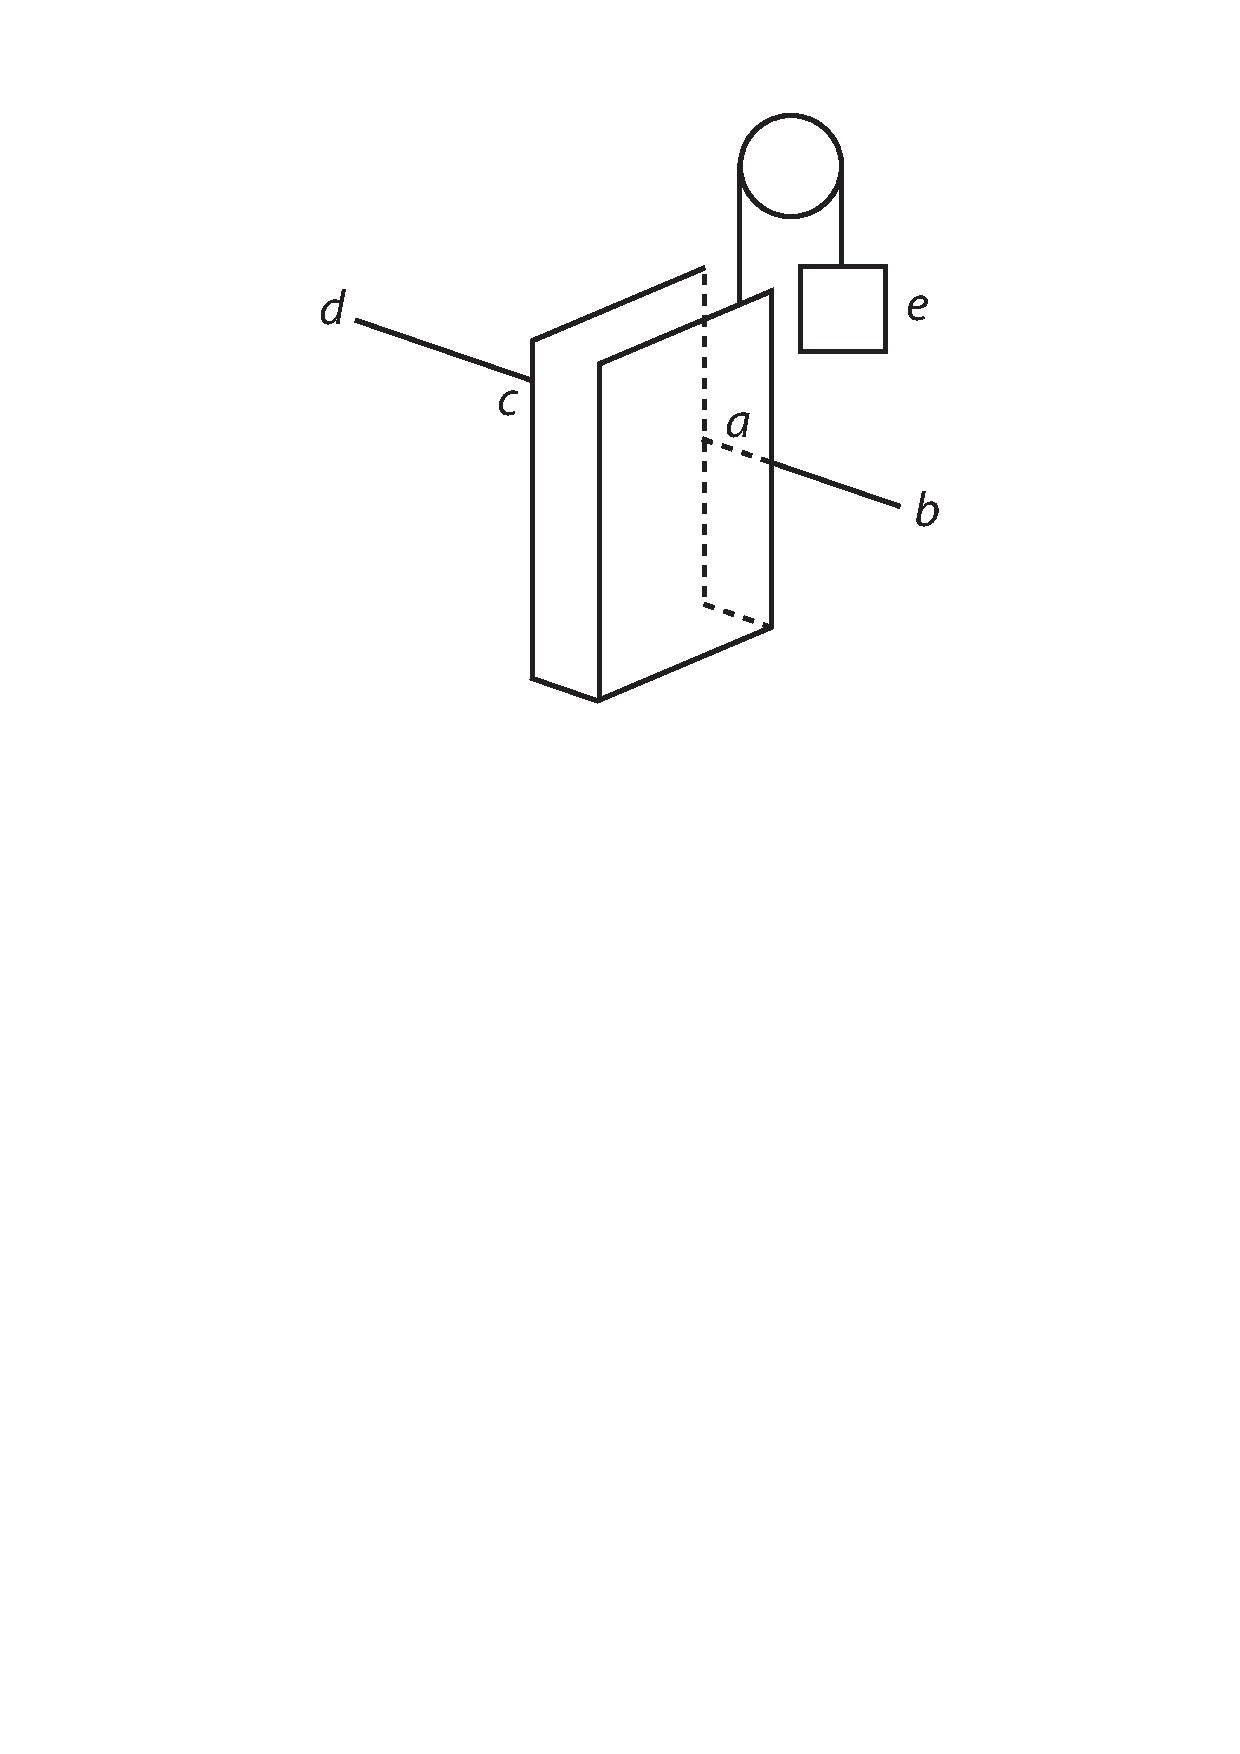
\includegraphics[%trim = -3mm -2mm 0mm 0mm, clip,
width=0.34\textwidth]
{images/lh03705_211v-d1.pdf},\hspace{25mm} {[\textit{Fig. 1}] %\vspace{4mm}
}]
\noindent
[211~v\textsuperscript{o}] \textso{De distractione.}
Sunto duae vis[,] altera applicata in $a$ conans\protect\index{Sachverzeichnis}{vis conans} versus $b$, altera applicata in $c$ conans versus $d$. Et vis $ab$ alligata est tabulae\protect\index{Sachverzeichnis}{tabula} $a$, vis $cd$ tabulae $c$.
{Tabulae\reversemarginpar\marginnote{\scriptsize\hspace{-13mm}15}} autem $a$ et $c$ non aliter junctae sunt, quam \edtext{filo,\protect\index{Sachverzeichnis}{filum} ita}{\lemma{\hspace{1.8mm}16\hspace{1.8mm}filo,}\killnumber\Bfootnote{\textit{(1)} quo \textit{(2)} ita \textit{L}}} ut inter distrahendum attrahatur filum, et attracto filo\protect\index{Sachverzeichnis}{filum} elevetur pondus\protect\index{Sachverzeichnis}{pondus} $e$.
\newline
\hspace*{7.5mm}%
Ponamus primum vires $cd$ \edtext{et}{\lemma{18\hspace{1.8mm}}\killnumber\Bfootnote{et \textit{erg. L}}} $ab$ esse aequales.
Tabula\protect\index{Sachverzeichnis}{tabula} $a$ habet conatum\protect\index{Sachverzeichnis}{conatus} $ab$.
Sed hunc perducere non potest ad motum, nisi {moveatur\reversemarginpar\marginnote{\scriptsize\hspace{-13mm}20}} quoque in $ab$ tabula $c$ vel elevetur pondus $e$.
Quodsi pondus\protect\index{Sachverzeichnis}{pondus} quoque $e$ conatui $ab$ sit aequale, et renitentia quoque seu contrarius conatus $cd$ aequalis sit cuilibet ipsorum: quid eventurum putamus?
\end{window}
%% [211~v\textsuperscript{o}]
%\begin{wrapfigure}[12]{l}{0.34\textwidth}
%\vspace{-5mm}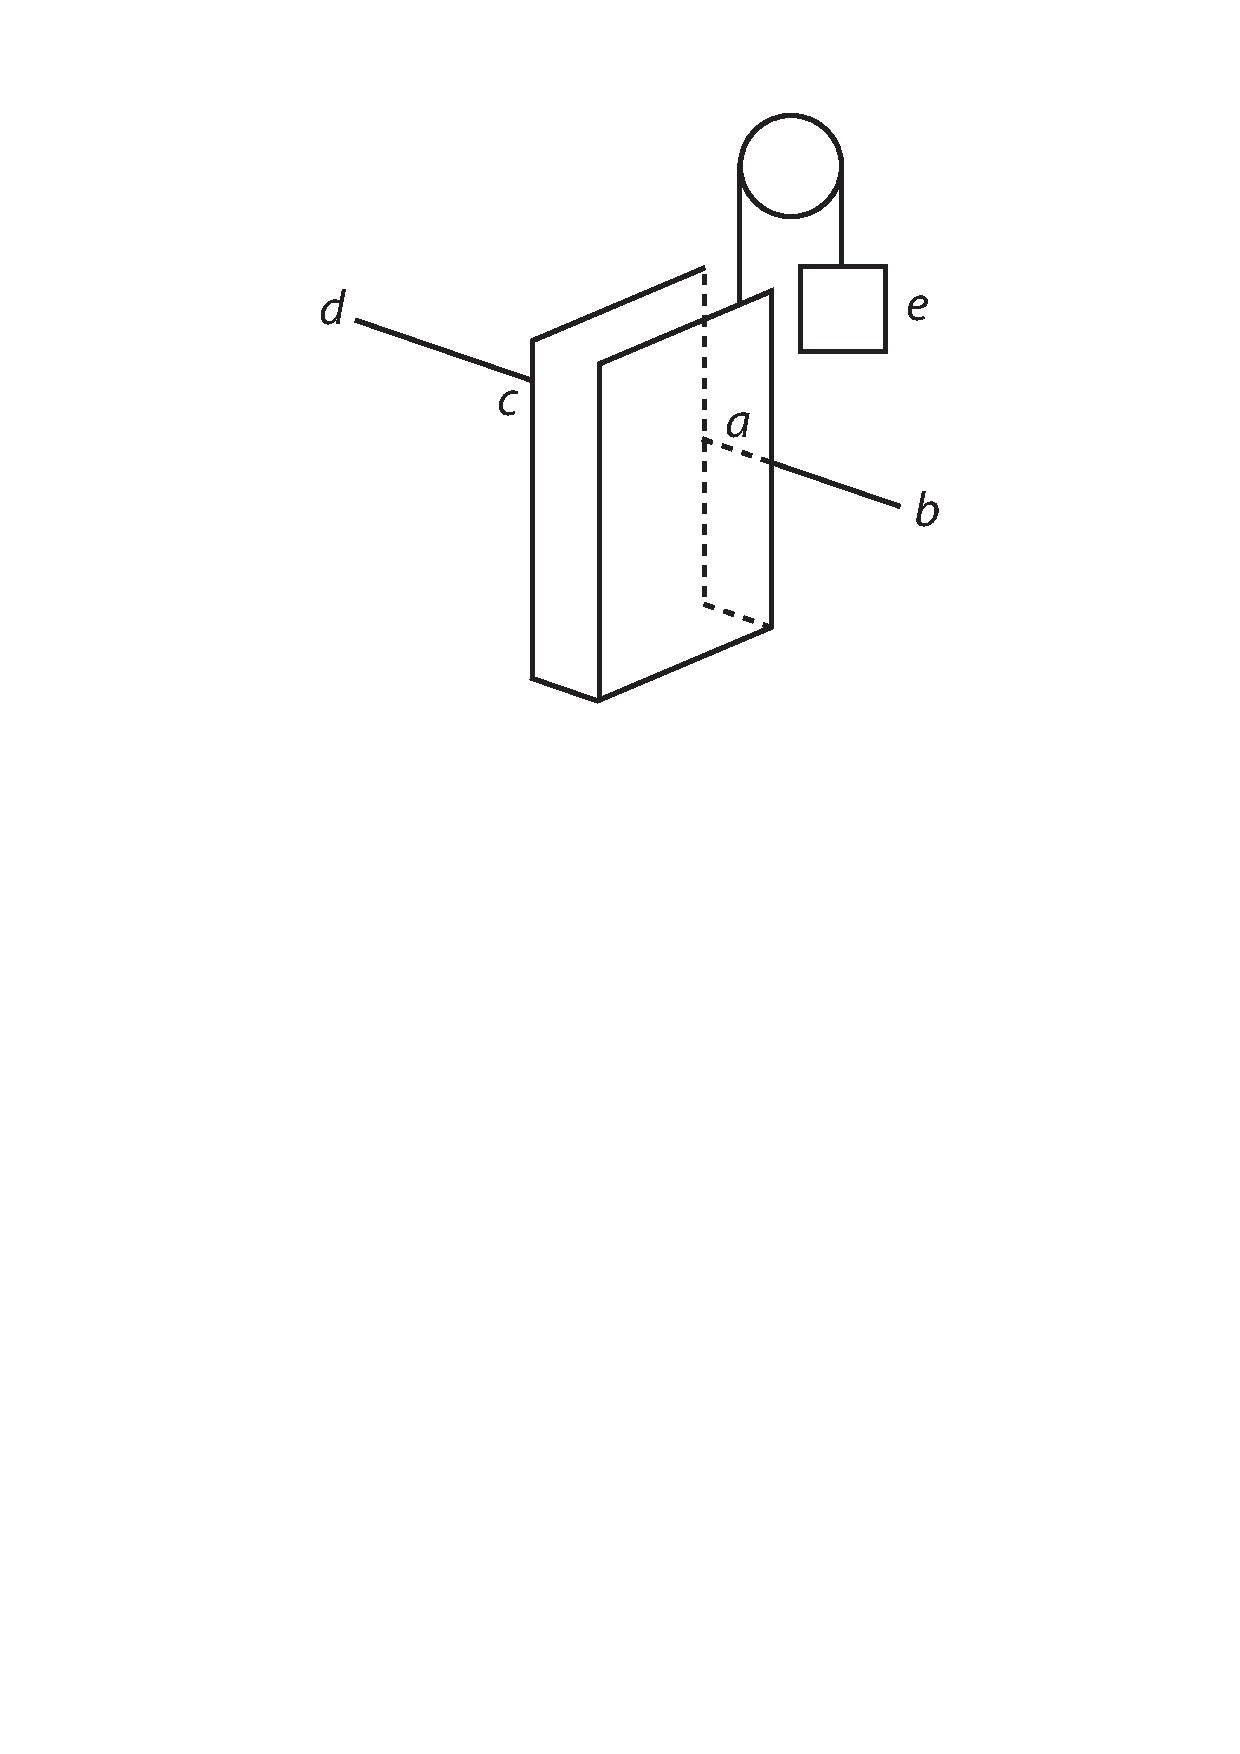
\includegraphics[trim = 0mm -3mm -5mm 0mm, clip, width=0.34\textwidth]{images/lh03705_211v-d1.pdf}\\
%\centering[\textit{Fig. 1}]
%\end{wrapfigure}
%211~v\textsuperscript{o}] \textso{De distractione.}
%Sunto duae vis[,] altera applicata in $a$ conans\protect\index{Sachverzeichnis}{vis conans} versus $b$, altera applicata in $c$ conans versus $d$. Et vis $ab$ alligata est tabulae\protect\index{Sachverzeichnis}{tabula} $a$, vis $cd$ tabulae $c$.
%Tabulae autem $a$ et $c$ non aliter junctae sunt, quam \edtext{filo,\protect\index{Sachverzeichnis}{filum} ita}{\lemma{filo,}\Bfootnote{\textit{(1)} quo \textit{(2)} ita \textit{L}}} ut inter distrahendum attrahatur filum, et attracto filo\protect\index{Sachverzeichnis}{filum} elevetur pondus\protect\index{Sachverzeichnis}{pondus} $e$.
%\newline
%\hspace*{7.5mm}%
%Ponamus primum vires $cd$ \edtext{et}{\lemma{}\Bfootnote{et \textit{erg. L}}} $ab$ esse aequales.
%Tabula\protect\index{Sachverzeichnis}{tabula} $a$ habet conatum\protect\index{Sachverzeichnis}{conatus} $ab$.
%Sed hunc perducere non potest ad motum, nisi moveatur quoque in $ab$ tabula $c$ vel elevetur pondus $e$.
%Quodsi pondus\protect\index{Sachverzeichnis}{pondus} quoque $e$ conatui $ab$ sit aequale, et renitentia quoque seu contrarius conatus $cd$ aequalis sit cuilibet ipsorum: quid eventurum putamus?
\pend
%\vspace{1.5em}
%\pstart%
%\noindent%
%\centering%
%\pend
%\newpage
\count\Afootins=1200
\count\Bfootins=1200
\count\Cfootins=1200
\pstart%
Manifestum \setline{24}est $a$ habere conatum $ab$ et \edtext{$c$ conatum $cd\ (= ab)$ et $a$}{\lemma{$c$ conatum $cd$}\Bfootnote{%
\textbar\ $(= ab)$ \textit{erg.} \textbar\ et $a$ \textit{L}}} conatum $cd\ (= ab),$ conditionaliter, si \edtext{pondus}{\lemma{pondus}\Bfootnote{\textit{erg. L}}} $e$ sit fortius conatu \edtext{$ab\ (=cd)$ et $c$ conatum $ab$}{\lemma{$ab\ (=cd)$}\Bfootnote{\textit{(1)} et $e$ \textit{(2)} conatum elevationis = conatui $ab$ \textit{(3)} et $c$ conatum $ab$ \textit{L}}} conditionaliter si pondus $e$ sit fortius conatu $cd$.
Et pondus $e$ conatum elevationis\protect\index{Sachverzeichnis}{conatus elevationis} ut $ab$, si $cd$ sit fortior $e$.
% \pend
% \pstart%
Et idem pondus $e$ conatum elevationis ut $cd$, si $ab$ sit \edlabel{distractione1}fortior $e$.
% \pend
% \pstart%
\edtext{\edlabel{distractione2}Ergo}{{\xxref{distractione1}{distractione2}}\lemma{fortior $e$.}\Bfootnote{\textit{(1)} Porro etiam $a$ habet conatum $ab$ si aut $cd$ aut $e$ in $c$ \textit{(2)} Ergo \textit{L}}} cum nec $ab$ nec $cd$ sit fortior $e$, nec $e$ vicissim fortior illis nullus erit conatus elevationis\protect\index{Sachverzeichnis}{conatus elevationis} in $e$ nec $ab$ in $c$ nec $cd$ in $a$.
\pend
\pstart%
Hinc jam sequitur etiam conatum $ab$ in $a$ et $cd$ in $c$ destrui.
Nam \edtext{neuter ad exitum}{\lemma{neuter}\Bfootnote{\textit{(1)} procedit, in \textit{(2)} ad exitum \textit{L}}} perduci potest, nisi aut oppositum accipiat conatum ipsius aut elevetur pondus $e$.\protect\index{Sachverzeichnis}{pondus}
Id est nisi aut pondus $e$ aut conatus $ab$ vel $cd$ sit fortior.
Sed cum sint aequales nihil horum eligi potest, ergo nec conatus $ab$ et $cd$ exitum reperiunt, et proinde manet \edlabel{distractione3}quies.
\pend
\pstart%
\edtext{Hinc intelligi \edlabel{distractione4}}{{\xxref{distractione3}{distractione4}}\lemma{quies.}\Bfootnote{\textit{(1)} Jam \textbar\ conatus \textit{erg.} \textbar\  $ab$ et $cd$ inaequales sunto major $ab$ minor $cd$ seu $ab = cd+F$ \textit{(2)} Hinc \textit{(a)} in genere \textit{(b)} intelligi \textit{L}}} \edtext{potest distrahentibus}{\lemma{}\Bfootnote{potest \textbar\ in \textit{gestr.} \textbar\ distrahentibus \textit{L}}} \edtext{aequalibus}{\lemma{}\Bfootnote{aequalibus \textit{erg. L}}} non nisi dimidium virium applicatarum agere in vinculum connectens.
Quod patet etiam, si Tibi \edtext{imagineris, alterum}{\lemma{imagineris,}\Bfootnote{\textit{(1)} quod \textit{(2)} alterum \textit{L}}} distrahendum non trahere sed reniti tantum, omnis enim renisus, retractio est.
\pend
\pstart%
Jam conatus $ab$ et $cd$ inaequales sunto major $ab$ minor $cd$ seu $ab = cd+F$.
Pondus\protect\index{Sachverzeichnis}{pondus} $e$ potest intelligi aequale aut alterutri aut neutri.
Si alterutri, aequale est aut majori, aut minori.
Si \edtext{majori, non sequetur}{\lemma{majori,}\Bfootnote{\textit{(1)} necessario \textit{(2)} non sequetur \textit{L}}} distractio,\protect\index{Sachverzeichnis}{distractio} sed abreptio trahentis oppositi una cum distrahendo.
Sed differentia virium\protect\index{Sachverzeichnis}{differentia virium} inter \edtext{distrahens majus}{\lemma{distrahens}\Bfootnote{\textit{(1)} ab \textit{(2)} majus \textit{L}}} et minus.
% \pend
% \pstart%
Si minori aequale est, itidem fiet abreptio non distractio, si minore minus est fiet distractio.\protect\index{Sachverzeichnis}{distractio}
Si majus non fiet.
\pend
\pstart%
Quaestio elegans, quando motus centralis, praevaleat libero seu absoluto.
Esto molendinum\protect\index{Sachverzeichnis}{molendinum} navi\protect\index{Sachverzeichnis}{navis} impositum, \edtext{quod circumactione}{\lemma{quod}\Bfootnote{\textit{(1)} circumacta \textit{(2)} circumactione \textit{L}}} sua remos\protect\index{Sachverzeichnis}{remus} agat.
Ventus\protect\index{Sachverzeichnis}{ventus} incidens in molendinum, quaeritur circumacturusne potius sit, an propulsurus, cum non sit locus fixus, circa quem fiat motus.
Et puto demonstrari posse, si valde onerata sit navis, facilius a vento circumactum iri quam propulsum.
Nam si ventus propellat circumactione\protect\index{Sachverzeichnis}{circumactio} molendini motus potentiae est celer, ponderis tardus.
At si propellat navem uterque motus est aeque celer, hinc fieri potest, ut quam navem\protect\index{Sachverzeichnis}{navis} ventus recta propellere non possit, seu quae ei renitatur, propulsurus sit circumagendo.
Et ut minor sit impulsus rectus,\protect\index{Sachverzeichnis}{impulsus} potest molendinum\protect\index{Sachverzeichnis}{molendinum} ubi centro vicinius, esse interruptum, ita decedet vi rectae plurimum, curvae parum.
Sed et opponi \edtext{possunt aquae in plagam}{\lemma{possunt}\Bfootnote{\textit{(1)} vento loco \textit{(2)} aquae in plagam \textit{L}}} quo ventus pellit coreacei quasi quidam sacci qui motu contra ventum\protect\index{Sachverzeichnis}{ventus} contrahuntur.
En quasi ancoras in ipsa aqua fixas.
\pend
\count\Afootins=1500
\count\Bfootins=1500
\count\Cfootins=1500